\chapter{Theory}

\section{General graph theory}

A graph $\mathcal{G} = \{V, E \} $ is defined by the set of its nodes $V$ and edges $E$. The edges forms the connections between nodes, and fora pair of nodes $(i,j)$ the corresponding edge may be denoted $e_{ij}$. We may define the neighbours to a certain node $v \in V$ as $N(v)$, which thus are the nodes $u \in V$ that are connected to $v$, $e_{vu} \neq 0$. Each node $v$ may also be associated with \textit{node features}, $x_v$. $x_v$ could be a vector, and can be seen as the properties of a node.

A graph is considered to be \textit{undirected} if the edges are undirected, $e_{ij} \equiv e_{ji}$, and \textit{directed} if the edges are directed, $e_{ij} \not\equiv e_{ji}$. Furthermore, a graph can either be \textit{binary} or \textit{weighted}. In a binary graph, edges are either present or not, whilst in a weighted graph each edge $e_{ij}$ is associated with a weight $w_{ij}$. \cite{source} Weights in a weighted graph may be interpreted differently depending on the application. They can be seen as the connection strength between devices in a cellular network, the flow of goods in a logistics setting, a distance metric etc.

The edges in a graph may be succinctly summarised in an \textit{adjacency matrix} $A$. $A$ is defined as

\begin{equation}
    A_{ij} = \begin{cases} \mbox{1,} & \mbox{if } e_{ij} \in E \\ \mbox{0,} & \mbox{otherwise} \end{cases}
    \label{eq:adjacencydefinition}
\end{equation}
In the case of a weighted graph, $A_{ij} = w_{ij}$. From definition \eqref{eq:adjacencydefinition} follows that undirected graphs have a symmetric adjacency matrix, $A_{ij} = A_{ji}$. In this work we mainly focus on the edges rather than the nodes of the brain networks, and thus adjacency matrices will be our primary way of representing graphs.



% \subsection{Graph classification}
% \subsection{Node classification}
% \subsection{regression}



\section{Graph Convolutional Neural Networks}
\label{sec:gcn}

Graph Convolutional Neural Networks (GCNs) are a class of neural networks that generalize the notion of convolutions from grid data to graph structured data \cite{wu_review}. Regular convolutional operations typically operate on structured grids of data, for instance the pixels in an image, where each grid point is only connected to its adjacent neighbours. This may not be the case in graph structured data, where any pair of nodes can be connected. This difference can be visualised as in figure \ref{fig:grid_graph_data}. 

\begin{figure}
    \centering
        \begin{subfigure}{.5\textwidth}
            \centering
            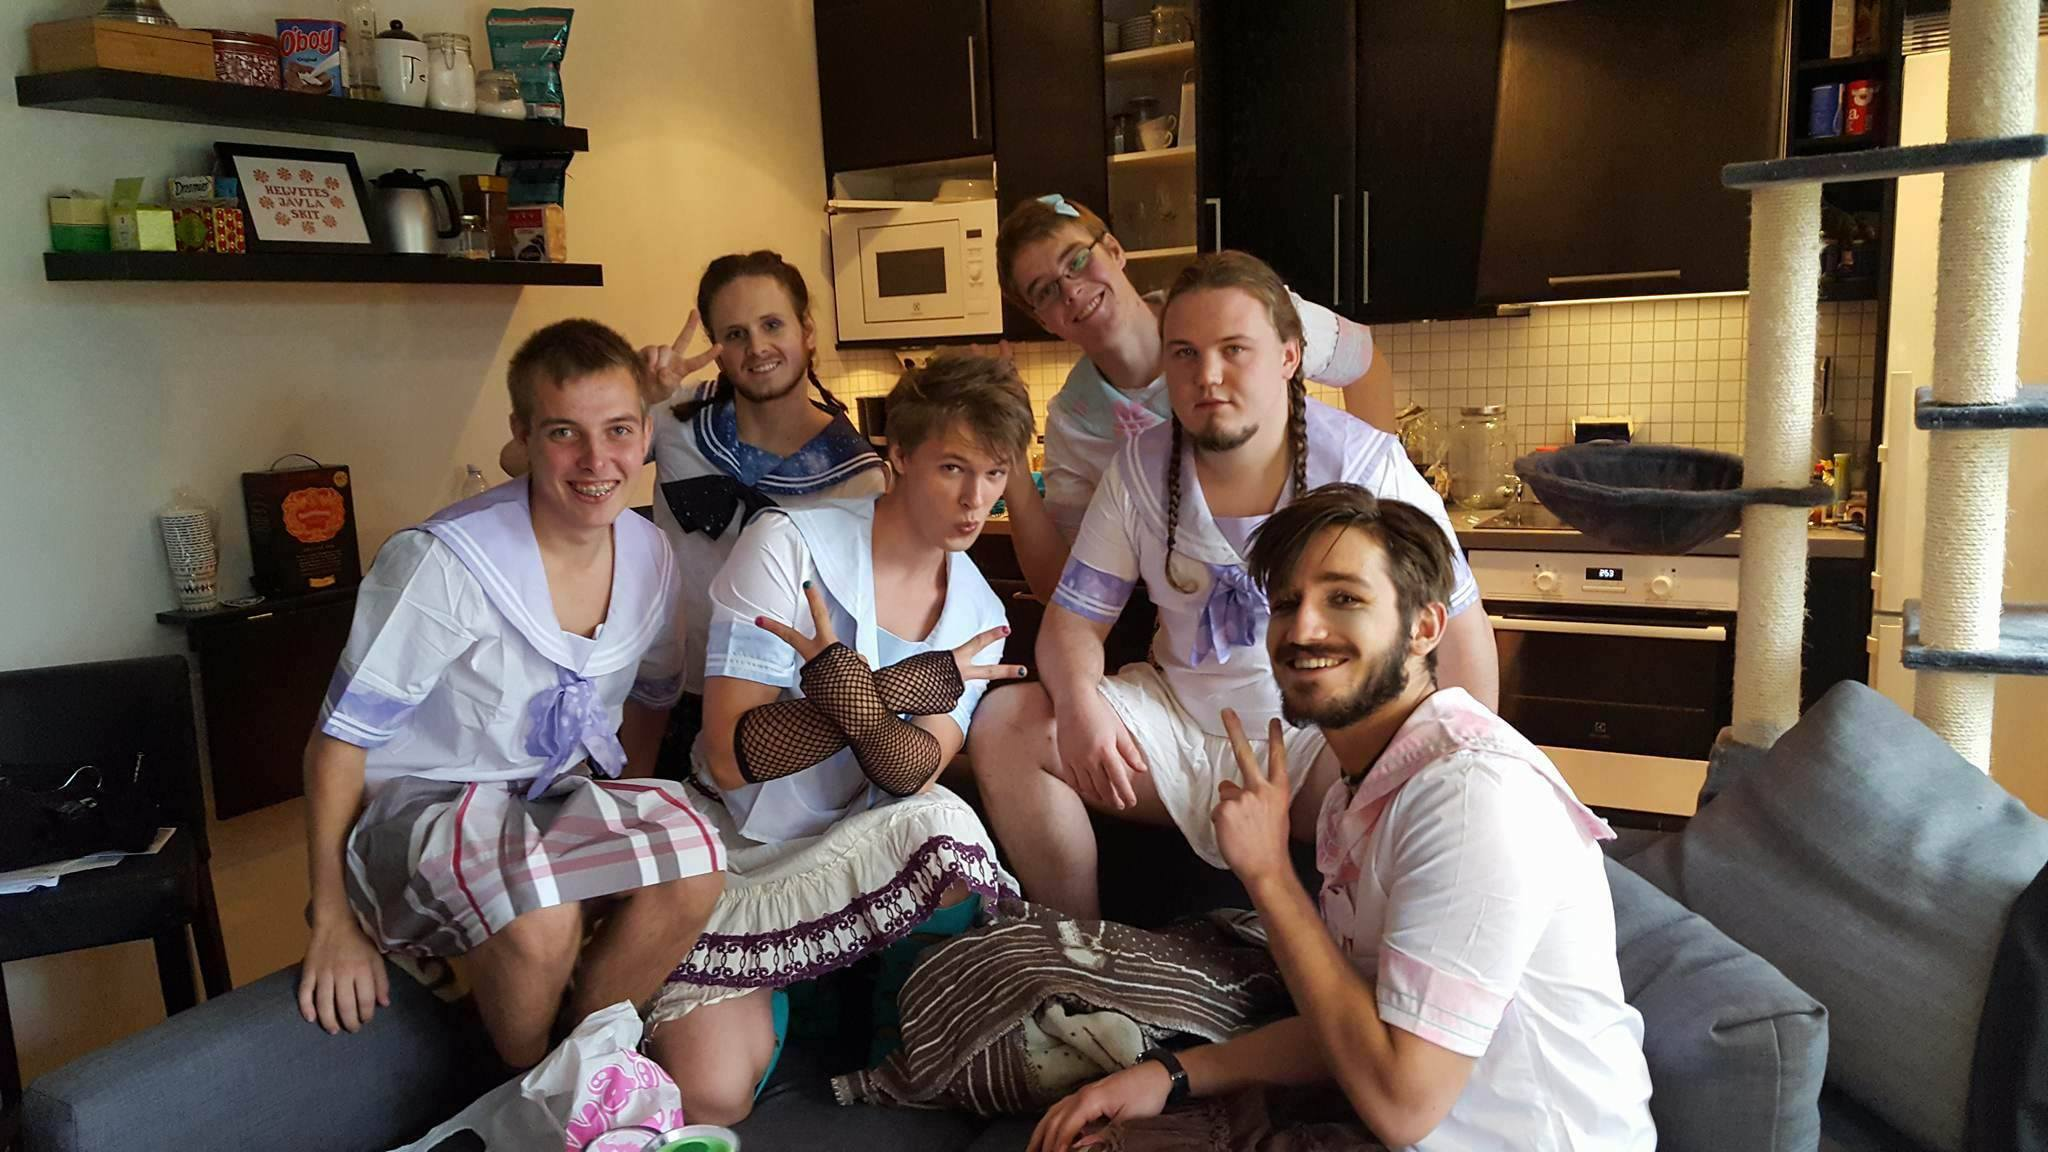
\includegraphics[width=.9\linewidth]{chapters/images_theory/placeholder.jpg}
            \caption{Grid data}
            \label{fig:grid_data}
        \end{subfigure}%
        \begin{subfigure}{.5\textwidth}
            \begin{center}
                \resizebox {0.9\linewidth} {!} {
                    

\tikzset{every picture/.style={line width=0.75pt}} %set default line width to 0.75pt        

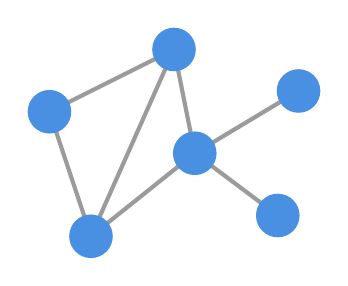
\begin{tikzpicture}[x=0.75pt,y=0.75pt,yscale=-1,xscale=1]
%uncomment if require: \path (0,140); %set diagram left start at 0, and has height of 140

%Straight Lines [id:da9529519883756523] 
\draw [color={rgb, 255:red, 155; green, 155; blue, 155 }  ,draw opacity=1 ][line width=1.5]    (90,70) -- (80,20) ;
%Straight Lines [id:da3936138198150927] 
\draw [color={rgb, 255:red, 155; green, 155; blue, 155 }  ,draw opacity=1 ][line width=1.5]    (40,110) -- (80,20) ;
%Straight Lines [id:da5548481843497526] 
\draw [color={rgb, 255:red, 155; green, 155; blue, 155 }  ,draw opacity=1 ][line width=1.5]    (20,50) -- (40,110) ;
%Straight Lines [id:da5819939155390126] 
\draw [color={rgb, 255:red, 155; green, 155; blue, 155 }  ,draw opacity=1 ][line width=1.5]    (90,70) -- (140,40) ;
%Straight Lines [id:da6057490474086391] 
\draw [color={rgb, 255:red, 155; green, 155; blue, 155 }  ,draw opacity=1 ][line width=1.5]    (20,50) -- (80,20) ;
%Straight Lines [id:da9589484835549189] 
\draw [color={rgb, 255:red, 155; green, 155; blue, 155 }  ,draw opacity=1 ][line width=1.5]    (90,70) -- (40,110) ;
%Straight Lines [id:da9003996251715192] 
\draw [color={rgb, 255:red, 155; green, 155; blue, 155 }  ,draw opacity=1 ][line width=1.5]    (90,70) -- (130,100) ;
%Shape: Circle [id:dp16002964648747287] 
\draw  [color={rgb, 255:red, 74; green, 144; blue, 226 }  ,draw opacity=1 ][fill={rgb, 255:red, 74; green, 144; blue, 226 }  ,fill opacity=1 ] (10,50) .. controls (10,44.48) and (14.48,40) .. (20,40) .. controls (25.52,40) and (30,44.48) .. (30,50) .. controls (30,55.52) and (25.52,60) .. (20,60) .. controls (14.48,60) and (10,55.52) .. (10,50) -- cycle ;
%Shape: Circle [id:dp6860897081767219] 
\draw  [color={rgb, 255:red, 74; green, 144; blue, 226 }  ,draw opacity=1 ][fill={rgb, 255:red, 74; green, 144; blue, 226 }  ,fill opacity=1 ] (30,110) .. controls (30,104.48) and (34.48,100) .. (40,100) .. controls (45.52,100) and (50,104.48) .. (50,110) .. controls (50,115.52) and (45.52,120) .. (40,120) .. controls (34.48,120) and (30,115.52) .. (30,110) -- cycle ;
%Shape: Circle [id:dp6864628521101095] 
\draw  [color={rgb, 255:red, 74; green, 144; blue, 226 }  ,draw opacity=1 ][fill={rgb, 255:red, 74; green, 144; blue, 226 }  ,fill opacity=1 ] (80,70) .. controls (80,64.48) and (84.48,60) .. (90,60) .. controls (95.52,60) and (100,64.48) .. (100,70) .. controls (100,75.52) and (95.52,80) .. (90,80) .. controls (84.48,80) and (80,75.52) .. (80,70) -- cycle ;
%Shape: Circle [id:dp3274470105344238] 
\draw  [color={rgb, 255:red, 74; green, 144; blue, 226 }  ,draw opacity=1 ][fill={rgb, 255:red, 74; green, 144; blue, 226 }  ,fill opacity=1 ] (120,100) .. controls (120,94.48) and (124.48,90) .. (130,90) .. controls (135.52,90) and (140,94.48) .. (140,100) .. controls (140,105.52) and (135.52,110) .. (130,110) .. controls (124.48,110) and (120,105.52) .. (120,100) -- cycle ;
%Shape: Circle [id:dp6718592584089527] 
\draw  [color={rgb, 255:red, 74; green, 144; blue, 226 }  ,draw opacity=1 ][fill={rgb, 255:red, 74; green, 144; blue, 226 }  ,fill opacity=1 ] (70,20) .. controls (70,14.48) and (74.48,10) .. (80,10) .. controls (85.52,10) and (90,14.48) .. (90,20) .. controls (90,25.52) and (85.52,30) .. (80,30) .. controls (74.48,30) and (70,25.52) .. (70,20) -- cycle ;
%Shape: Circle [id:dp3995705243055563] 
\draw  [color={rgb, 255:red, 74; green, 144; blue, 226 }  ,draw opacity=1 ][fill={rgb, 255:red, 74; green, 144; blue, 226 }  ,fill opacity=1 ] (130,40) .. controls (130,34.48) and (134.48,30) .. (140,30) .. controls (145.52,30) and (150,34.48) .. (150,40) .. controls (150,45.52) and (145.52,50) .. (140,50) .. controls (134.48,50) and (130,45.52) .. (130,40) -- cycle ;




\end{tikzpicture}

                }
            \end{center}
            \caption{Graph data}
            \label{fig:graph_dad}
        \end{subfigure}
    \caption{Comparison between grid structured and graph structured data }
    \label{fig:grid_graph_data}
\end{figure}

We begin by first discussing the concept of convolutions in the graph domain, and how they can implemented in a computationally efficient manner. We then present a layer-wise propagation rule for a graph convolutional layer based on this implementation of convolutions. Finally, we discuss graph convolutional layers from the viewpoint of a heuristic interpretation known as \textit{message passing}.

\subsection{Convolutions in the graph domain}

Consider an undirected graph $\mathcal{G} = (\mathcal{V}, \mathcal{E})$ with $N$ nodes and adjacency matrix $A$. The degree matrix $D$ to $\mathcal{G}$ is defined as 
\begin{equation}
    D_{ij} = \begin{cases} \sum_j A_{ij}, & \mbox{if } i = j \\ \mbox{0,} & \mbox{otherwise} \end{cases}.
    \label{eq:degreematrixdefinition}
\end{equation}
We can now define the graph Laplacian $L= D-A $ for the graph $\mathcal{G}$. $L$ can be normalized according to 
\begin{equation}
    L_\text{norm} = D^{-1/2} L D^{-1/2} =  I_N - D^{-1/2} A D^{-1/2},
    \label{eq:normalized_graph_laplacian}
\end{equation}
where $I_N$ is the $N$x$N$ identity matrix. In the following we assume that the graph Laplacian $L$ is normalized according to equation \eqref{eq:normalized_graph_laplacian}.

Having defined the graph laplacian $L$, we may now turn to convolutions. The convolution of the signal $x$ with a filter $g_\theta = diag(\theta)$, parametrized by a parameter $\theta \in R^N$ in the Fourier domain, can be written as 

\begin{equation}
    g_\theta * x = U g_\theta U^T x,
    \label{eq:graph_convolution}
\end{equation}
where $U$ is an orthogonal matrix containing the eigenvectors of $L$. However, performing convolutions using equation \ref{eq:graph_convolution} may be computationally intractable in practice, partly because multiplication with $U$ is $\mathcal{O}(N^2)$ and partly because calculating $U$ requires the eigendecomposition of $L$, which may be very computationally expensive for large graphs \cite{kipf_semi_supervised}. A way around this problem is discussed in Kipf et. al \cite{kipf_semi_supervised}, in which the filter $g_\theta$ in equation \ref{eq:graph_convolution} is approximated to $g_{\theta'}$ using an expansion in Chebyshev polynomials $T_k(x)$:s. To the $K^{\text{th}}$ order, the convolution $g_\theta * x$ may be written as 

\begin{equation}
    g_{\theta'} * x \approx \sum_{k=0}^K \theta'_k T_k(\tilde{L})x,
    \label{eq:convolution_approximation}
\end{equation}
where $\tilde{L} =  \frac{2}{\lambda_{\text{max}}}L - I_N$, and $\lambda_{\text{max}}$ is the largest eigenvalue of $L$. $\theta'_k$ is here a vector of Chebyshev coefficients, which in the context of machine learning corresponds to trainable parameters. The Chebyshev polynomials are recursively defined as 
\begin{equation}
    T_k(x) = 2xT_{k-1}(x) - T_{k-2}(x), \hspace{10px} T_0(x) = 1, \hspace{5px} T_1(x) = x.
\end{equation}

The interpretation of equation \eqref{eq:convolution_approximation} is that the convolution is $K^{\text{th}}$ order local, i.e. that a convolution considers each node and their $K^{\text{th}}$ order neighbors, i.e. the neighbours that are at most $K$ steps away in the graph. 


\subsection{Layer-wise propagation rule}

Following Kipf et. al \cite{kipf_semi_supervised}, we set $K=1$ in equation \eqref{eq:convolution_approximation}, limiting the convolution to only consider a node ($k=0$) and its closest neighbours ($k=1$). This results in 

\begin{equation}
    g_{\theta'} * x \approx \theta_0' x + \theta_1' \left( \frac{2}{\lambda_{\text{max}}}L - I_N \right)x.
    \label{eq:k1_approximation_step1}
\end{equation}
We may further simplify equation \eqref{eq:k1_approximation_step1} by fixing the maximum eigenvalue of $L$, $\lambda_{\text{max}} = 2$. This is a change of scale, but one that the neural network should be able to adapt to during training. We then obtain

\begin{equation}
    g_{\theta'} * x \approx \theta_0' x + \theta_1' \left(L - I_N \right)x = \theta_0' x - \theta_1' D^{-1/2}AD^{-1/2}x ,
    \label{eq:k1_approximation_step2}
\end{equation}
and by setting a single trainable parameter $\theta = \theta_0' = -\theta_1'$ we arrive at 
\begin{equation}
    g_{\theta'} * x \approx \theta \left(I_N + D^{-1/2}AD^{-1/2} \right)x. 
    \label{eq:k1_approximation_step3}
\end{equation}
$I_N + D^{-1/2}AD^{-1/2}$ has eigenvalues in the range $[0, 2]$, and thus implementing convolutions as in equation \eqref{eq:k1_approximation_step3} in a neural network may lead to exploding or vanishing gradients. This problem can be avoided using a \textit{renormalization trick}:

\begin{equation}
    I_N + D^{-1/2}AD^{-1/2} \rightarrow \tilde{D}^{-1/2} \tilde{A} \tilde{D}^{-1/2}
    \label{eq:renormalization_trick}
\end{equation}
where $\tilde{A} = A + I_N$ and $\tilde{D} = \sum_j \tilde{A}_{ij}$.
We may now generalize this expression for a convolution operation to a signal $X \in \mathbb{R}^{N \times C}$, defined on the $N$ nodes of the graph and with a $C$-dimensional feature vector for each node. The signal $X$ thus has $C$ input channels. Furthermore, let the convolution apply $F$ filters to the $C$ input channels. The application of such a convolution can thus be written

\begin{equation}
    Z = \tilde{D}^{-1/2} \tilde{A} \tilde{D}^{-1/2} X \Theta,
    \label{eq:propagation_rule}
\end{equation}
with $\Theta \in \mathbb{R}^{C\times F}$ being a matrix of filter parameters and $Z \in \mathbb{R}^{N\times F}$ as the convolved signal. This propagation rule in equation \eqref{eq:propagation_rule}, when paired with an activation function $\sigma$ such that $H = \sigma\left(Z \right)$, forms the basis for a GCN. 

Recall that we in order to arrive at this expression for a convolution set $K=1$ in the Chebyshev polynomial expansion in equation \eqref{eq:convolution_approximation}. As discussed, this limits the convolution to only consider each node and its closest neighbours. Furthermore, the approximation becomes a linear function in $L$, i.e. a function that is linear in the graph spectral domain. These two points may seem to be limitations in the representational strength of the graph convolutional layer, however this is not necessarily the case \cite{kipf_semi_supervised}. First, larger neighbourhoods can be convolved over by stacking multiple layers, with the first layer considering a node and its neghbours, the second layer considering the neighbours neighbours and so on. Secondly, keeping the representation linear in $L$ actually makes it more flexible, since it is not dependant on the explicit parametrization given by the Chebyshev polynomials. Combined, a deep GCN consisting of several stacked graph convolutional layers paired with possibly non-linear activation functions $\sigma$ can still model a rich class of convolutional filter functions, whilst keeping computational costs low. 


\subsection{Message passing as an approximation of spectral theory}
\label{subsec:message_passing}

As discussed in the previous section, a graph convolutional layer aggregates the features $x_v$ for each node $v$ and $x_u$ for all of its neighbours $u \in N(v)$, with larger neighbourhoods being considered by stacking multiple layers. Heuristically, a graph convolutional layer can thus be seen to perform a sort of \textit{message passing}, in that each node receives messages (aggregates features) from all of its closest neighbours. This can be seen by studying the propagation rule in equation \eqref{eq:propagation_rule} for a single node $i$ and a single filter channel $F=1$, and explicitly rewriting it as a sum: 

\begin{equation}
    z_i = \sum_k \theta_k \left(\hat{A}_{ii} x_{ik} + \sum_{j \neq i} \hat{A}_{ij} x_{jk} \right)
\end{equation}
where $z_i$ is the activation for node $i$, $x_{ik}$ corresponds to feature $k$ for node $i$, $\theta_k$ is the trainable weight for feature $k$ and $\hat{A} = \tilde{D}^{-1/2} \tilde{A} \tilde{D}^{-1/2}$. $\hat{A}_{ij}$ is only non-zero for the nodes $j$ which are directly connected to node $i$, and thus only the nodes that are first-order neighbours to node $i$ will contribute to the sum $\sum_{j \neq i} \hat{A}_{ij} x_{jk}$. $\hat{A}_{ii}$ is a self-connection, since the $i$:th node is a zero-order neighbour to itself.
By interpreting the features $x_{ik}$ as a form of \textit{message}, the expression $\hat{A}_{ii} x_{ik} + \sum_{j \neq i} \hat{A}_{ij} x_{jk}$ can be seen as an aggregation of messages between a node's current state $x_{ik}$ and those of its neighbours $x_{jk}\left.\right\rvert_{j\neq i}$. Furthermore, in a weighted graph $\hat{A}_{ij}$ may be interpreted as the connection strength between nodes, and thus the contribution of each node can be seen as weighted by that strength. Finally, these contributions are summed up for all features $k$ with their corresponding trainable weight $\theta_k$ to yield the node's activation $z_i$. In this manner information can flow through the graph, and by stacking multiple GCN layers the information can spread over successively larger neighbourhoods. See figure \ref{fig:message_passing} for a visual representation of how the ``messages'' are passed to node $i$ from it's neighbours.

\begin{figure}[H]
    \centering
    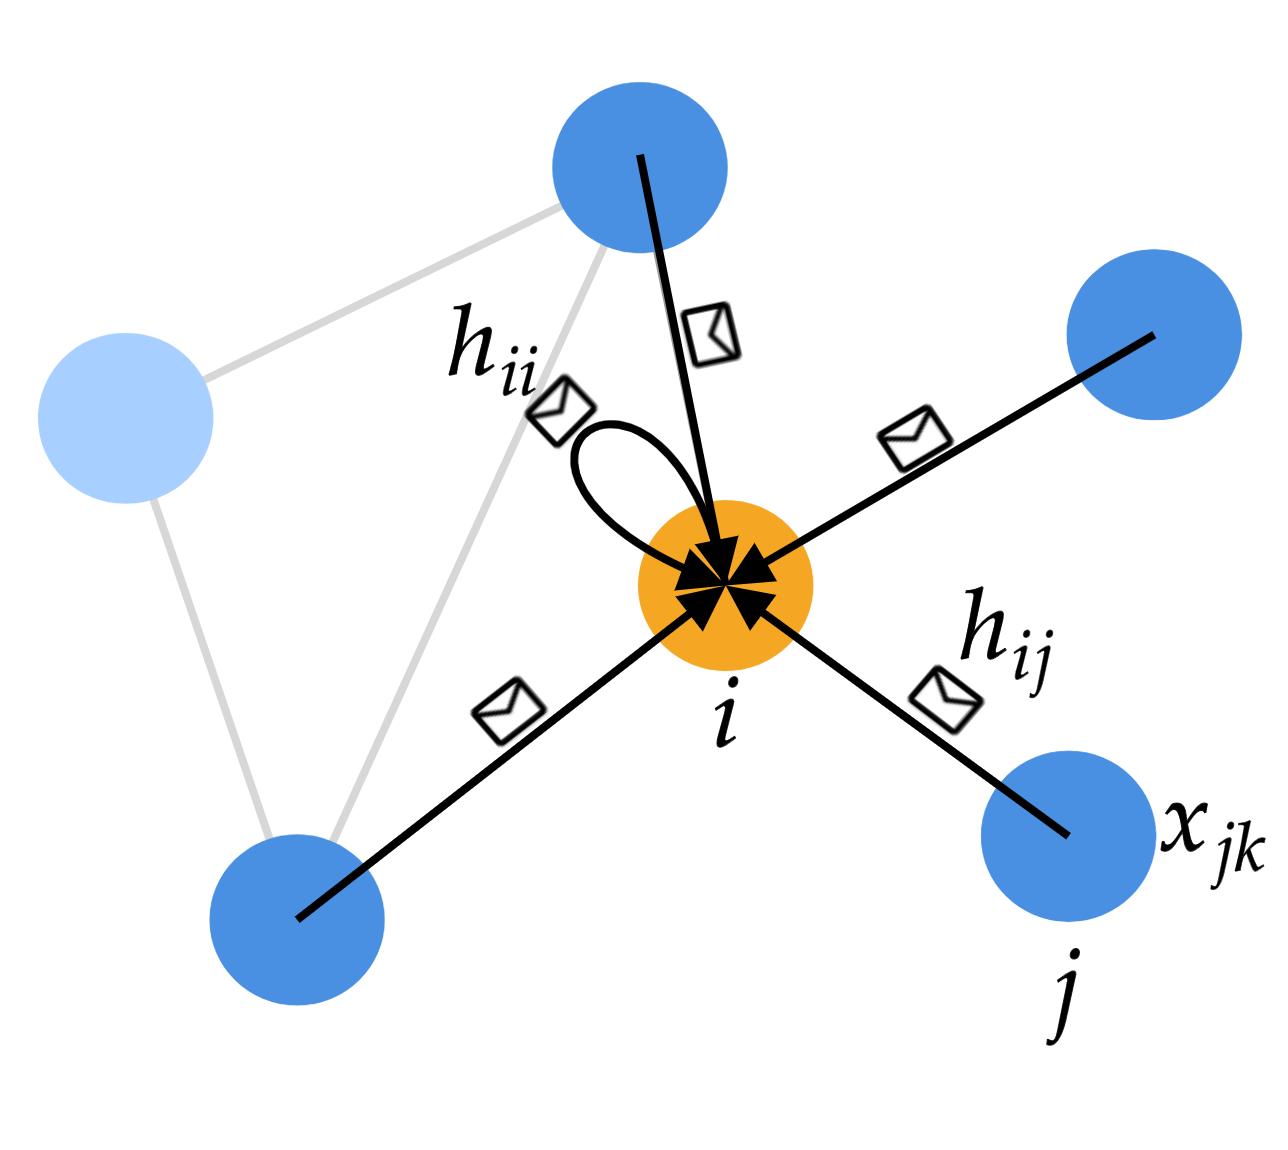
\includegraphics[width=0.5\linewidth]{chapters/images_theory/message_passing.png}
    \caption{A schematic representation of the message passing interpretation of a GCN layer. The messages $x_{jk}$ are weighted by the connection strength $\hat{A}_{ij}$ when sent from node $j$ to node $i$. All contribtions from node $i$'s neighbours are aggregated in this manner, and then multiplied by the weight $\theta_k$.}
    \label{fig:message_passing}
\end{figure}


%  The term $A_{ii} x_{ik}$ corresponds to the current state of node $i$:s, which is aggregated with the contributions from the sum $\sum_{j \neq i} A_{ij} x_{jk}$. 
% The idea behind GCNs is to aggregate the features $x_v$ for each node $v$ and $x_u$ for all of its neighbours $u \in N(v)$, and thus successively share information across the graph. Heuristically, this can be seen as a form of \textit{message passing}, in which each node communicates its features to all of its neighbours. 

\section{Machine learning on graphs}
\label{sec:ml_on_graphs}

Graphs are very versatile in storing data, and are thus abundant in many areas of science. It is thus interesting how one incorporates them into the framework of machine learning. Specifically, how does one formulate a problem to suitably be solved using machine learning on graphs? 

%% TODO TIKZ
% \begin{center}
%     \resizebox {\textwidth} {!} {
%         

\tikzset{every picture/.style={line width=0.75pt}} %set default line width to 0.75pt        

\begin{tikzpicture}[x=0.75pt,y=0.75pt,yscale=-1,xscale=1]
%uncomment if require: \path (0,208); %set diagram left start at 0, and has height of 208

%Straight Lines [id:da08555474507907834] 
\draw [color={rgb, 255:red, 155; green, 155; blue, 155 }  ,draw opacity=1 ][line width=1.5]    (144.81,72.72) -- (139.59,141.54) ;
%Straight Lines [id:da7854957979705237] 
\draw [color={rgb, 255:red, 155; green, 155; blue, 155 }  ,draw opacity=1 ][line width=1.5]    (144.81,72.72) -- (170.94,112.87) ;
%Straight Lines [id:da5355133218247532] 
\draw [color={rgb, 255:red, 155; green, 155; blue, 155 }  ,draw opacity=1 ][line width=1.5]    (139.59,141.54) -- (170.94,112.87) ;
%Straight Lines [id:da7379744038533278] 
\draw [color={rgb, 255:red, 155; green, 155; blue, 155 }  ,draw opacity=1 ][line width=1.5]    (197.06,72.72) -- (170.94,112.87) ;
%Straight Lines [id:da3385355935149281] 
\draw [color={rgb, 255:red, 155; green, 155; blue, 155 }  ,draw opacity=1 ][line width=1.5]    (197.06,72.72) -- (259.74,84.19) ;
%Straight Lines [id:da6697105472921161] 
\draw [color={rgb, 255:red, 155; green, 155; blue, 155 }  ,draw opacity=1 ][line width=1.5]    (197.06,72.72) -- (223.18,107.13) ;
%Straight Lines [id:da44213623412323666] 
\draw [color={rgb, 255:red, 155; green, 155; blue, 155 }  ,draw opacity=1 ][line width=1.5]    (249.3,135.81) -- (197.06,147.28) ;
%Straight Lines [id:da340514368127399] 
\draw [color={rgb, 255:red, 155; green, 155; blue, 155 }  ,draw opacity=1 ][line width=1.5]    (223.18,107.13) -- (249.3,135.81) ;
%Straight Lines [id:da07640316595483987] 
\draw [color={rgb, 255:red, 155; green, 155; blue, 155 }  ,draw opacity=1 ][line width=1.5]    (259.74,84.19) -- (249.3,135.81) ;
%Shape: Trapezoid [id:dp2008857707852969] 
\draw  [color={rgb, 255:red, 255; green, 255; blue, 255 }  ,draw opacity=1 ][fill={rgb, 255:red, 255; green, 255; blue, 255 }  ,fill opacity=1 ] (254.52,89.93) -- (257.66,78.46) -- (261.83,78.46) -- (264.97,89.93) -- cycle ;
%Image [id:dp4810218304838956] 
\draw (259.74,84.19) node  {\includegraphics[width=15.67pt,height=17.2pt]{ClbFhBFF8L-person-blue-36dp-filled.svg}};

%Straight Lines [id:da17683212694460426] 
\draw [color={rgb, 255:red, 155; green, 155; blue, 155 }  ,draw opacity=1 ][line width=1.5]    (139.59,141.54) -- (197.06,147.28) ;
%Shape: Trapezoid [id:dp06527551163848622] 
\draw  [color={rgb, 255:red, 255; green, 255; blue, 255 }  ,draw opacity=1 ][fill={rgb, 255:red, 255; green, 255; blue, 255 }  ,fill opacity=1 ] (191.83,153.01) -- (194.97,141.54) -- (199.15,141.54) -- (202.28,153.01) -- cycle ;
%Image [id:dp24121370862546265] 
\draw (197.06,147.28) node  {\includegraphics[width=15.67pt,height=17.2pt]{ClbFhBFF8L-person-blue-36dp-filled.svg}};

%Shape: Trapezoid [id:dp6568478256577734] 
\draw  [color={rgb, 255:red, 255; green, 255; blue, 255 }  ,draw opacity=1 ][fill={rgb, 255:red, 255; green, 255; blue, 255 }  ,fill opacity=1 ] (134.37,147.28) -- (137.5,135.81) -- (141.68,135.81) -- (144.81,147.28) -- cycle ;
%Image [id:dp6219332582048571] 
\draw (139.59,141.54) node  {\includegraphics[width=15.67pt,height=17.2pt]{ClbFhBFF8L-person-blue-36dp-filled.svg}};

%Straight Lines [id:da3735509406273694] 
\draw [color={rgb, 255:red, 155; green, 155; blue, 155 }  ,draw opacity=1 ][line width=1.5]    (170.94,112.87) -- (223.18,107.13) ;
%Shape: Trapezoid [id:dp8065935750477351] 
\draw  [color={rgb, 255:red, 255; green, 255; blue, 255 }  ,draw opacity=1 ][fill={rgb, 255:red, 255; green, 255; blue, 255 }  ,fill opacity=1 ] (217.95,112.87) -- (221.09,101.4) -- (225.27,101.4) -- (228.4,112.87) -- cycle ;
%Image [id:dp45354658145120497] 
\draw (223.18,107.13) node  {\includegraphics[width=15.67pt,height=17.2pt]{ClbFhBFF8L-person-blue-36dp-filled.svg}};

%Straight Lines [id:da3264902727456349] 
\draw [color={rgb, 255:red, 155; green, 155; blue, 155 }  ,draw opacity=1 ][line width=1.5]    (249.3,135.81) -- (170.94,112.87) ;
%Shape: Trapezoid [id:dp866311010615511] 
\draw  [color={rgb, 255:red, 255; green, 255; blue, 255 }  ,draw opacity=1 ][fill={rgb, 255:red, 255; green, 255; blue, 255 }  ,fill opacity=1 ] (244.07,141.54) -- (247.21,130.07) -- (251.39,130.07) -- (254.52,141.54) -- cycle ;
%Image [id:dp8422386634219512] 
\draw (249.3,135.81) node  {\includegraphics[width=15.67pt,height=17.2pt]{ClbFhBFF8L-person-blue-36dp-filled.svg}};

%Shape: Trapezoid [id:dp8073086406080059] 
\draw  [color={rgb, 255:red, 255; green, 255; blue, 255 }  ,draw opacity=1 ][fill={rgb, 255:red, 255; green, 255; blue, 255 }  ,fill opacity=1 ] (165.71,118.6) -- (168.85,107.13) -- (173.02,107.13) -- (176.16,118.6) -- cycle ;
%Image [id:dp888581341362926] 
\draw (170.94,112.87) node  {\includegraphics[width=15.67pt,height=17.2pt]{ClbFhBFF8L-person-blue-36dp-filled.svg}};

%Straight Lines [id:da4374734471484929] 
\draw [color={rgb, 255:red, 155; green, 155; blue, 155 }  ,draw opacity=1 ][line width=1.5]    (144.81,72.72) -- (197.06,72.72) ;
%Shape: Trapezoid [id:dp17137240691479927] 
\draw  [color={rgb, 255:red, 255; green, 255; blue, 255 }  ,draw opacity=1 ][fill={rgb, 255:red, 255; green, 255; blue, 255 }  ,fill opacity=1 ] (191.83,78.46) -- (194.97,66.99) -- (199.15,66.99) -- (202.28,78.46) -- cycle ;
%Image [id:dp3965566139299834] 
\draw (197.06,72.72) node  {\includegraphics[width=15.67pt,height=17.2pt]{ClbFhBFF8L-person-blue-36dp-filled.svg}};

%Shape: Trapezoid [id:dp7022737407670283] 
\draw  [color={rgb, 255:red, 255; green, 255; blue, 255 }  ,draw opacity=1 ][fill={rgb, 255:red, 255; green, 255; blue, 255 }  ,fill opacity=1 ] (139.59,78.46) -- (142.72,66.99) -- (146.9,66.99) -- (150.04,78.46) -- cycle ;
%Image [id:dp7793647929632923] 
\draw (144.81,72.72) node  {\includegraphics[width=15.67pt,height=17.2pt]{ClbFhBFF8L-person-blue-36dp-filled.svg}};


%Rounded Rect [id:dp2921184592491468] 
\draw   (120,74) .. controls (120,60.75) and (130.75,50) .. (144,50) -- (250.11,50) .. controls (263.37,50) and (274.11,60.75) .. (274.11,74) -- (274.11,146) .. controls (274.11,159.25) and (263.37,170) .. (250.11,170) -- (144,170) .. controls (130.75,170) and (120,159.25) .. (120,146) -- cycle ;

%Straight Lines [id:da280482111384722] 
\draw    (474,110) -- (414,110) ;
%Rounded Rect [id:dp23949785762119213] 
\draw   (324.11,92) .. controls (324.11,85.37) and (329.48,80) .. (336.11,80) -- (402.11,80) .. controls (408.74,80) and (414.11,85.37) .. (414.11,92) -- (414.11,128) .. controls (414.11,134.63) and (408.74,140) .. (402.11,140) -- (336.11,140) .. controls (329.48,140) and (324.11,134.63) .. (324.11,128) -- cycle ;

%Straight Lines [id:da18593803425726807] 
\draw    (324.11,110) -- (274.11,110) ;
%Rounded Rect [id:dp14732801608712798] 
\draw   (474,98) .. controls (474,93.58) and (477.58,90) .. (482,90) -- (576,90) .. controls (580.42,90) and (584,93.58) .. (584,98) -- (584,122) .. controls (584,126.42) and (580.42,130) .. (576,130) -- (482,130) .. controls (477.58,130) and (474,126.42) .. (474,122) -- cycle ;
%Image [id:dp556169067273697] 
\draw (45.6,68) node  {\includegraphics[width=30pt,height=30pt]{ClbFhBFF8L-person-blue-36dp-filled.svg}};
%Image [id:dp2790482390271307] 
\draw (45.6,108) node  {\includegraphics[width=30pt,height=30pt]{ClbFhBFF8L-person-blue-36dp-filled.svg}};
%Image [id:dp9089881134245916] 
\draw (45.6,148) node  {\includegraphics[width=30pt,height=30pt]{ClbFhBFF8L-person-blue-36dp-filled.svg}};
%Rounded Rect [id:dp06427479999848584] 
\draw  [dash pattern={on 4.5pt off 4.5pt}] (12,61.6) .. controls (12,54.09) and (18.09,48) .. (25.6,48) -- (66.4,48) .. controls (73.91,48) and (80,54.09) .. (80,61.6) -- (80,156.4) .. controls (80,163.91) and (73.91,170) .. (66.4,170) -- (25.6,170) .. controls (18.09,170) and (12,163.91) .. (12,156.4) -- cycle ;
%Straight Lines [id:da8499548057058206] 
\draw    (120,110) -- (80,110) ;

% Text Node
\draw (340.11,96) node [anchor=north west][inner sep=0.75pt]   [align=left] {{\Large Model}};
% Text Node
\draw (439,89.4) node [anchor=north west][inner sep=0.75pt]    {$y$};
% Text Node
\draw (295.11,90.4) node [anchor=north west][inner sep=0.75pt]    {$X$};
% Text Node
\draw (483,99) node [anchor=north west][inner sep=0.75pt]   [align=left] {{\large Predictions}};


\end{tikzpicture}

%     }
% \end{center}

\begin{figure}[H]
    \centering
        \begin{subfigure}{.5\textwidth}
            \centering
            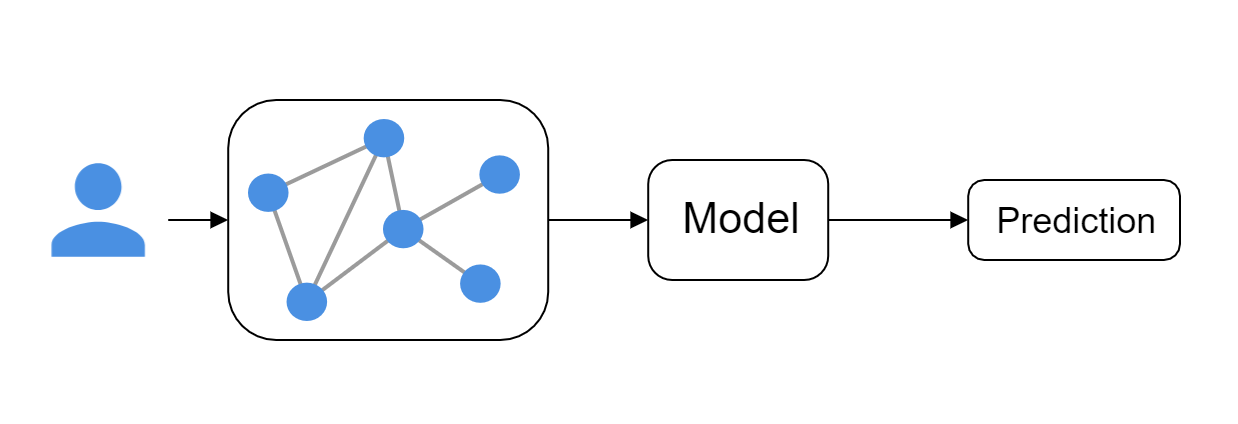
\includegraphics[width=.9\linewidth]{chapters/images_theory/graph_classification.png}
            \caption{Graph classification}
            \label{fig:graph_classification}
        \end{subfigure}%
        \begin{subfigure}{.5\textwidth}
            \centering
            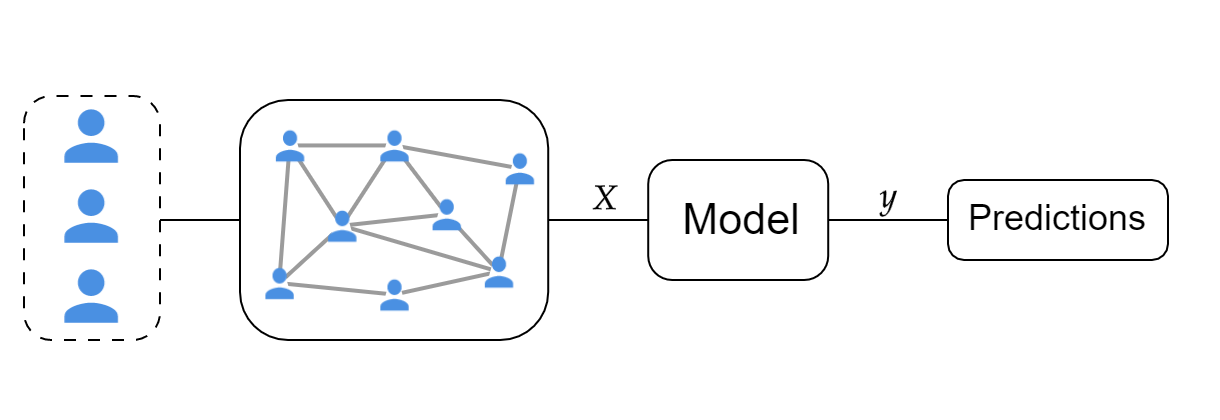
\includegraphics[width=.9\linewidth]{chapters/images_theory/node_classification.png}
            \caption{Node classification}
            \label{fig:node_classification}
        \end{subfigure}
    \caption{Schematic representations of node and graph classification. }
    \label{fig:graph_and_node_class}
\end{figure}

One common class of problems is \textit{graph classification}. As the name implies, given a graph $\mathcal{G}$ the task is to classify it as belonging to one of several classes. Another class of problem is \textit{node classification}. The task here is to classify each node in the set of nodes $V$ belonging to the graph $\mathcal{G} = \{V, E \}$. The schematics of graph classification and node classification can be seen in figures \ref{fig:graph_classification} and \ref{fig:node_classification} respectively. Graph and node classification can be generalised to graph and node \textit{regression}, in which a continuous value is predicted for each graph or node, respectively. We will in the following refer to graph and node classification/regression as graph or node \textit{inference}.

In the context of neuroscience, graph inference can be important when you have one graph per subject. These subject-specific graphs could for instance represent the brain structure of the subject. The task is then to predict some property for each subject given their graph. Node inference could be be important both on a subject level and a population level. For subject level graphs, one could infer node level properties, such as the properties of a part of a subject's brain. On a population level, one may represent the entire population as a single \textit{population graph}, in which each node corresponds to an individual. The set of nodes $V$ thus corresponds to the population, and the edges $E$ relate all individuals to each other. The idea behind this construction is that the nodes contain features related to each subject, whilst the edges contain information on how they relate to one another \cite{stankeviciute}. The set of edges $E$ can be calculated from a similarity measure, which thus encodes information on the similarity between subjects. The similarity measure greatly shapes the resulting population graph, and should be chosen with the specific application in mind. Common machine learning tasks on a population graph include predicting properties for each subject in the graph, i.e. a node inference problem. In neuroscience, these properties could be the age or sex of each subject.  

\section{Graph theory in neuroscience}
Ta upp relaterade arbeten och knyt ihop med introduction inför metoden. E.g. Jansson sandström, stankeviciute.


\section{Analysis}
\subsection{Model analysis/evaluation}
\subsection{Zorro}
The Zorro algorithm is an algorithm for determine which nodes and features are important for a model performing semi-supervised node classification. This means that the dataset consists of one big graph with one adjacency matrix and one feature matrix.

%This algorithm is by the writers introduced for analysing models performing semi-supervised node classification. This means that the dataset consists of one big graph with one adjacency matrix and one feature matrix. Since we are doing graphs classification where each subject has a unique adjacency matrix some alterations must be done to the algorithm. First we, in a big picture, describe how the Zorro algorithm works and then what alterations have been made by us.

To describe the Zorro algorithm a model $\Phi_n(X,A)$ is introduced which takes as input an adjacency $A$ matrix and a feature matrix $X$ and gives a prediction for each node $n$. The general idea is to replace the feature matrix $X$ by noise and then reintroduce nodes and features which makes the model prediction similar to the original. The way the noise is introduced is by 
\begin{equation*}
    Y_s = X \odot S + Z \odot (1- S), \quad Z \sim \mathcal{N}, 
\end{equation*}
where $S = \{V, F\}$ is refereed to as a explanation where the nodes $V$ and features $F$ is unmasked. The noise $\mathcal{N}$ is proposed by the authors of \cite{} to be set to the distribution of the dataset. The prediction of the model $\Phi$ on the masked data is then $\Phi_n(Y_s, A)$. To evaluate an explanation $S$ i.e. if a node and feature is important for the prediction of a specific node the fidelity of the explanation is calculated by
\begin{equation*}
    \mathcal{F}(S) = \mathbb{E}_{Y_s|Z\sim\mathcal{N}}[1_{\Phi_n(X,A) = \Phi_n(Y_s,A)}].
\end{equation*}
The fidelity of an explanation is a measure of how likely it is for a model with a masked dataset to give the same prediction as model with the original dataset. The algorithm then consists by iterative add the node or feature that increases the fidelity the most until the fidelity of an explanation is higher then a hyper parameter $\tau$. 

\subsection{Saliency mappings etc.}


